\documentclass[12pt]{article}
\usepackage[utf8]{inputenc}
\usepackage{amsmath}
\usepackage{amssymb}
\usepackage{titlesec}
\usepackage{listings}
\usepackage{xcolor}
\usepackage{hyperref}
\usepackage{graphicx}
\usepackage{booktabs}

\lstdefinestyle{mystyle}{
    backgroundcolor=\color{white}, % Set background color
    basicstyle=\ttfamily\footnotesize, % Use a typewriter font
    commentstyle=\color{gray},     % Comment color
    keywordstyle=\color{blue},     % Keyword color
    numberstyle=\tiny\color{gray}, % Line number color
    stringstyle=\color{red},       % String color
    breaklines=true,               % Automatically break long lines
    frame=single,                  % Draw a frame around the code
    numbers=left,                  % Line numbers on the left
    numbersep=5pt,                 % Distance of line numbers from code
    showspaces=false,              % Don't show spaces
    showstringspaces=false,        % Don't show spaces in strings
    showtabs=false,                % Don't show tabs
    tabsize=4                      % Set default tab size
}

% Apply the custom style
\lstset{style=mystyle}

\usepackage{geometry}
\geometry{a4paper, margin=1in}

\usepackage[backend=biber, style=numeric, citestyle=numeric]{biblatex} % Load biblatex with the numeric style
\addbibresource{references.bib} % Specify the database of bibliographic references
\usepackage{hyperref} % For clickable links

\title{Simple TTS using a vocoder-like method}
\author{Davide Giuseppe Griffon}
\date{}

\titleformat{\paragraph}
{\normalfont\normalsize\bfseries}{\theparagraph}{1em}{}
\titlespacing*{\paragraph}
{0pt}{3.25ex plus 1ex minus .2ex}{1.5ex plus .2ex}

\begin{document}

\maketitle

\begin{abstract}
    This document serves as the report for the second task in the "Natural Language Processing" course completed by student Davide Giuseppe Griffon at Vilnius University as part of the Master's program in Data Science.
\end{abstract}

\tableofcontents

\newpage

\section{Introduction}

In the rapidly evolving field of Natural Language Processing (NLP), Text-to-Speech (TTS) synthesis serves as a fundamental technology that bridges the gap between written and spoken language. The primary objective of TTS systems is to generate clear and natural-sounding speech from text, enhancing accessibility for a broader audience, including individuals with visual impairments or speech disorders. Achieving effective TTS synthesis requires an interdisciplinary approach, combining insights from linguistics, digital signal processing, and machine learning to emulate the complexities of human speech production.

\subsection{Vocoders}
Since the first attempts in this area, many modern models aiming to synthesize human speech have relied on vocoders. The \textit{vocoder}, short for ``voice encoder,'' is a critical component that transforms intermediate linguistic or acoustic representations into audible speech waveforms. This technology ensures that synthesized speech is not only intelligible but also carries the natural prosodic features that make human speech expressive and engaging. Understanding the role and evolution of vocoders is essential for appreciating their impact on modern speech synthesis technologies.

\subsubsection{Traditional Parametric Vocoders}

Traditional parametric vocoders, such as STRAIGHT and WORLD, process speech signals using specific algorithms based on acoustic analysis. They operate by decomposing the speech into key acoustic features. In particular they extract:

\begin{itemize}
    \item \textbf{Spectral Envelope}: This is a smooth curve representing the resonant frequencies (formants) of the vocal tract over time. The spectral envelope characterizes the timbre or color of the speech, reflecting how the shape and movements of the vocal tract affect the sound produced.
    
    \item \textbf{F0 (Fundamental Frequency)}: The fundamental frequency corresponds to the pitch or perceived frequency of the voice. It determines the intonation and melody of speech, playing a vital role in conveying meaning, emotion, and emphasis through variations in pitch.
    
    \item \textbf{Aperiodicity (or Noise Components)}: These components capture the noise and non-periodic parts of the speech signal. They are essential for accurately reproducing unvoiced sounds like fricatives (/s/, /f/), which are characterized by turbulent airflow rather than vocal cord vibrations.
\end{itemize}

After extracting these features, the vocoders synthesize a new waveform by reconstructing the signal based on the analyzed parameters. Although both STRAIGHT and WORLD aim to produce natural-sounding speech from this decomposition, they utilize different algorithms and methods for the analysis and synthesis stages.

These parametric vocoders are valued for their computational efficiency and precise control over speech parameters, making them suitable for real-time applications and environments with limited computational resources. However, a common drawback is that the speech they produce often sounds robotic and lacks the natural expressiveness and subtle nuances inherent in human speech.

\subsubsection{Neural-Based Vocoders}

The advent of neural vocoders, such as WaveNet and HiFi-GAN, has revolutionized the field by leveraging deep learning techniques to generate highly natural and human-like speech. These models learn complex mappings between acoustic features and waveforms from extensive datasets, capturing subtle nuances in prosody and emotion. While neural vocoders significantly enhance the naturalness of synthesized speech, they demand substantial computational resources and large training datasets.



% -------------------------------------------------------------------------------------------------
% -------------------------------------------------------------------------------------------------
% -------------------------------------------------------------------------------------------------



\section{Methodology}

In this section, I describe the step-by-step process I followed to implement a vocoder-like method for speech synthesis. The goal is to transform an input speech signal into a Mel spectrogram using the Short-Time Fourier Transform (STFT) and Mel scaling, and then reconstruct the waveform from this spectrogram. The final steps involve saving the reconstructed waveform as a \texttt{.wav} file and analyzing its quality using both objective and subjective methods.

Implementation note: Unlike the first assignment, where I chose not to rely on the \texttt{librosa} library and used only \texttt{numpy}, in this assignment I decided to use only \texttt{librosa} because it already contains many useful functions.

\subsection{Transforming the Speech Signal into a Mel Spectrogram}

The first step involves converting the input audio waveform, which is a time-domain signal, into a frequency-domain representation called a Mel spectrogram. This transformation is essential because it allows us to analyze the frequency content of the audio over time, which is crucial for speech processing.

I started by applying the Short-Time Fourier Transform (STFT) to the audio signal. The STFT divides the signal into short, overlapping time frames, computes the Fourier Transform for each frame, and applies a windowing function to smooth each frame. For this step, I used the \texttt{librosa} function \texttt{librosa.stft}, which performs this task in a single step. While I could have broken this process down into several steps—framing, windowing, and Fourier transformation—this \texttt{librosa} function is so convenient that I chose this simplified approach.

The magnitude of the complex spectrogram obtained from the STFT is then converted to power, and the resulting power signal is transformed into a Mel spectrogram using the function \texttt{librosa.feature.melspectrogram}, which computes a Mel-scaled spectrogram.

The Mel spectrogram is computed by mapping the frequencies of the magnitude spectrogram onto the Mel scale using a set of triangular filters, known as the Mel filter bank. This results in a two-dimensional representation where one axis represents time, and the other represents frequency on the Mel scale.

\subsubsection{Why Mel Spectrogram?}
Humans are better at detecting differences in lower frequencies than in higher frequencies. For example, we can easily tell the difference between 500 Hz and 1000 Hz, but would hardly detect a difference between 10,000 Hz and 10,500 Hz, even though the difference between the two pairs is the same. The Mel scale is designed to align more closely with how humans perceive pitch, giving greater resolution to lower frequencies and compressing higher frequencies.


\subsection{Reconstructing the Waveform from the Mel Spectrogram}

Reconstructing the original audio waveform from the Mel spectrogram is a complex task. For instance, the Mel spectrogram lacks phase information, which is essential for accurate signal reconstruction. Additionally, the Mel scaling compresses the frequency representation, adding further complexity to this process. To manage these challenges, I relied on existing \textit{librosa} functions, specifically:

\begin{itemize}
    \item \texttt{librosa.feature.inverse.mel\_to\_stft}, which approximates the STFT magnitude from a Mel power spectrogram.
    \item \texttt{librosa.griffinlim}, which performs an approximate magnitude spectrogram inversion using the "fast" Griffin-Lim algorithm.
\end{itemize}

After these two steps, the reconstructed audio waveform is obtained and can be easily saved as a new \texttt{.wav} file. For this step, I used the \texttt{write} function from the \textit{python-soundfile} audio library.



% -------------------------------------------------------------------------------------------------
% -------------------------------------------------------------------------------------------------
% -------------------------------------------------------------------------------------------------



\section{Analysis and Results}
For this assessment, I evaluated three sources of data to examine how differences in audio files affect performance. The sources I used are:

\begin{itemize}
    \item \textbf{Generated audio files}: This dataset is the same one I used in Assignment 1, consisting of 10 words generated with Lovo.ai.
    \item \textbf{AudioMNIST}: A dataset containing audio samples of spoken digits (0-9) from 60 different speakers.
    \item \textbf{Recorded}: Audio files I recorded using my own voice.
\end{itemize}

Using these diverse datasets allowed me to evaluate my project in a more comprehensive way.

Once the audio is reconstructed from the Mel spectrogram, it’s time to evaluate the quality of the reconstruction. In the codebase, provided in the appendix along with the Github repository, I wrote a few functions to plot the Mel spectrogram, the waveforms (both original and generated), and the F0 contour. The analysis of these plots provides an idea of how well this project was implemented. Following this "subjective" analysis of intermediate steps, I conducted both objective and subjective evaluations of the reconstructed audio files.

\subsection{Analysis of Intermediate Steps}

Analyzing intermediate steps is essential to ensure the process is on the right track before producing the final result, the reconstructed audio file. A clear way to evaluate intermediate results is by visualizing them in plotted form. I wrote three utility functions to plot these results: \texttt{save\_mel\_spectrogram\_plot}, \texttt{save\_waveforms}, and \texttt{save\_f0\_contour}.

\subsubsection{Mel Spectrogram}
Plotting the Mel spectrogram is straightforward; in this case, I used the function \\ \texttt{librosa.display.specshow}. In Figure~\ref{fig:melspec_zero}, the Mel spectrogram of the word "Zero" from the AudioMNIST dataset is shown.

\begin{figure}[h]
    \centering
    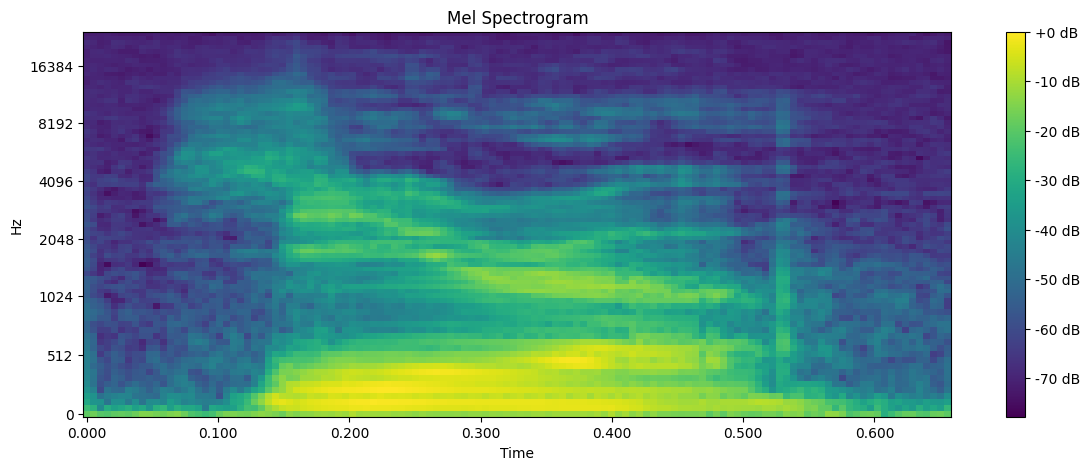
\includegraphics[width=\linewidth]{melspec_zero.png}
    \caption{Mel spectrogram of the word "Zero" from AudioMNIST}
    \label{fig:melspec_zero}
\end{figure}

\subsubsection{Waveform}
To display the waveform, I used the simple \texttt{librosa.display.waveshow} function from \texttt{librosa}. In Figure~\ref{fig:wav_accents_recorded}, the waveform of the word "Accents," recorded by me, is displayed for both the original and reconstructed versions. As shown, the two plots are quite similar.

\begin{figure}[h]
    \centering
    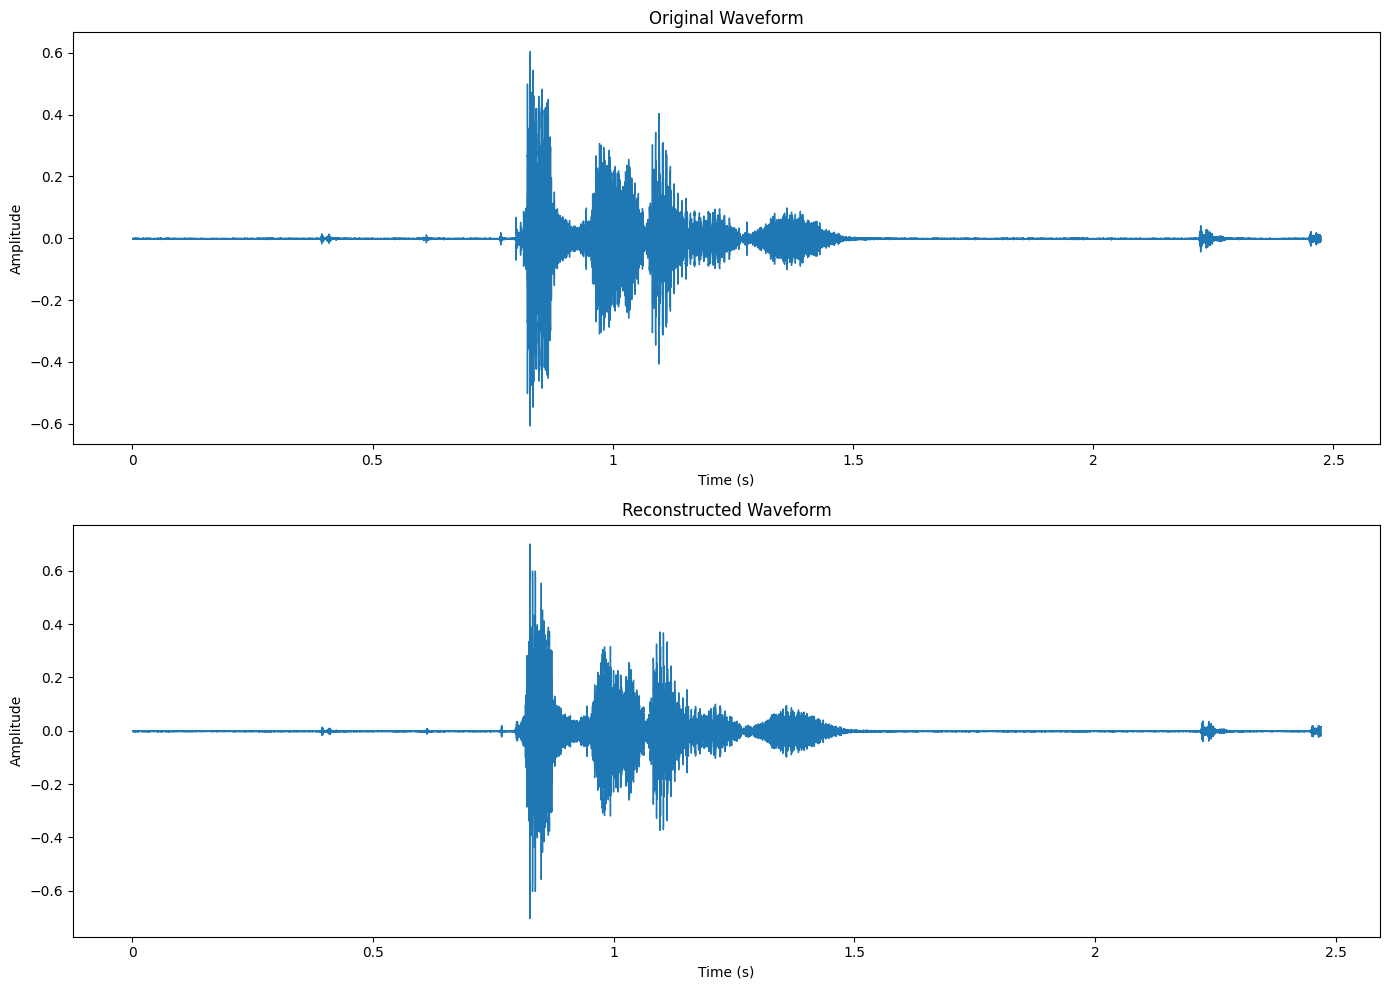
\includegraphics[width=\linewidth]{waveform_accents_recorded.png}
    \caption{Waveform of the word "Accents" recorded by me: original and reconstructed}
    \label{fig:wav_accents_recorded}
\end{figure}

\subsubsection{F0 Contour}
The fundamental frequency (F0) of a speech signal represents pitch—the perceptual characteristic that determines how high or low a sound is perceived. Pitch is essential for conveying meaning and emotion in speech. In an acoustic framework, intonation refers to the variation in pitch, which enhances the expressive quality of spoken language.

To calculate F0, I used \texttt{librosa.pyin}, which estimates it using a specialized algorithm. In Figure~\ref{fig:f0_phonetics}, the original and reconstructed F0 contours of the word "Phonetics" from the generated audio dataset are displayed. As illustrated, the F0 of the reconstructed version closely resembles the original.

\begin{figure}[h]
    \centering
    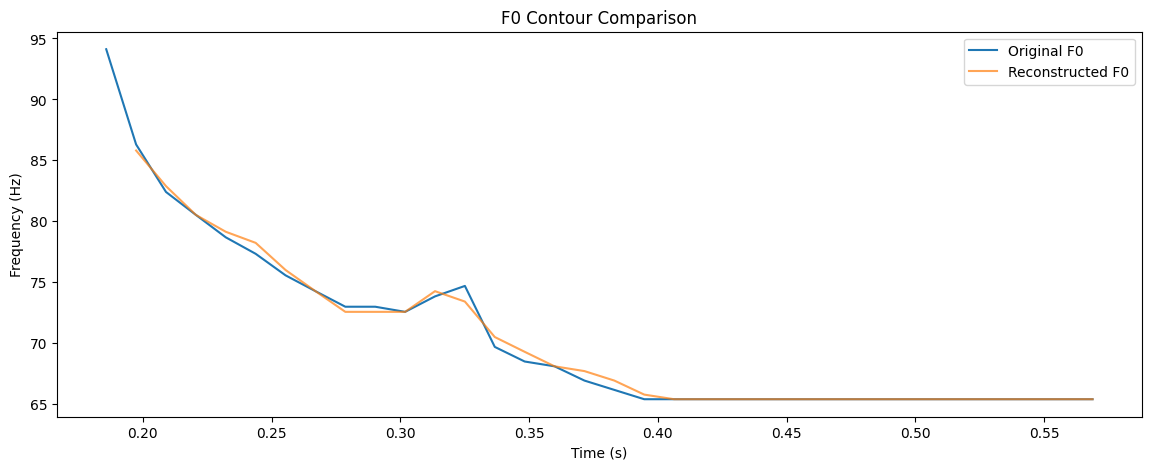
\includegraphics[width=\linewidth]{f0_phonetics.png}
    \caption{F0 contours of the word "Phonetics" from the generated audio dataset: original and reconstructed}
    \label{fig:f0_phonetics}
\end{figure}


\subsection{Analysis of the Reconstructed Audio}

Finally, I evaluated the reconstructed audio files using both objective and subjective methods.

\subsubsection{Objective Analysis}

The Perceptual Evaluation of Speech Quality (PESQ) is an objective measure designed to assess the quality of speech signals by comparing a degraded version—such as one that has been synthesized, enhanced, or compressed—to a clean reference signal. This approach replicates the human auditory system to estimate how people would perceive the quality of the impaired signal. The PESQ algorithm is sophisticated, involving multiple signal processing stages, including time alignment, frequency analysis, and cognitive modeling.

To perform PESQ, I used the Python library \texttt{pesq}. Below are some example logs:

\begin{verbatim}
Processing file: tts/audio_tts/mnist_0_27_8.wav
PESQ Score: 2.812911033630371

Processing file: tts/audio_tts/recorded_accents.wav
PESQ Score: 3.6831583976745605

Processing file: tts/audio_tts/generated_detect_tim_hardway_12.wav
PESQ Score: 2.4536759853363037
\end{verbatim}

In all PESQ evaluations I performed, the scores ranged between 2 and 4. This indicates that the final reconstructed audio has decent quality, but it is not perfect.

\subsubsection{Subjective Analysis}

Generally, the quality of the reconstructed audio is fairly decent, as established by the PESQ scores. I generally agree with the PESQ evaluations. In almost all the samples, I can recognize that the generated audio was reconstructed artificially, especially the audio from the generated dataset. In about one third of the generated audio samples, there is noticeable robotic distortion, but in all cases, the word is recognizable.


\section{Conclusions}

This project implemented a basic vocoder-like method for speech synthesis by converting speech signals into Mel spectrograms and reconstructing the waveforms. While the reconstructed audio retained intelligibility, it exhibited noticeable artifacts and sounded less natural than the original recordings. PESQ scores ranging from 2 to 4 reflected this moderate similarity. The imperfections are probably derived from the loss of phase information during the conversion to Mel spectrograms.

Modern neural vocoders like WaveNet and HiFi-GAN overcome these limitations by using deep learning to model both magnitude and phase directly from data. They capture complex patterns in speech signals, producing highly natural and realistic audio. Unlike traditional methods, these neural vocoders generate the waveform end-to-end, resulting in superior quality.

In summary, while method used in this project provides a foundational understanding of speech synthesis, it highlights the challenges of traditional vocoder techniques.


\newpage


% -------------------------------------------------------------------------------------------------
% -------------------------------------------------------------------------------------------------
% -------------------------------------------------------------------------------------------------

\section{Appendix: Codebase}

The codebase is fully avaible on Github, but covenience it's reported in this appendix for a quick review.

\begin{lstlisting}[language=Python, basicstyle=\fontsize{8}{9}\ttfamily]
from pathlib import Path
from typing import Tuple
import numpy as np
import librosa
import librosa.display
import matplotlib.pyplot as plt
import soundfile as sf
from scipy.io import wavfile
from pesq import pesq
import os


# Constants
N_FFT = 1024
HOP_LENGHT = 256
N_MELS = 80


def compute_mel_spectrogram(
    audio_data: np.ndarray,
    sample_rate: int,
) -> np.ndarray:
    """
    Compute the Mel spectrogram from an audio signal.
    """
    # Compute STFT to get the complex spectrogram
    stft = librosa.stft(audio_data, n_fft=N_FFT, hop_length=HOP_LENGHT)
    # Compute the magnitude spectrogram
    magnitude_spectrogram = np.abs(stft)
    # Convert the amplitude spectrogram to power spectrogram
    power_spectrogram = magnitude_spectrogram**2
    # Compute the Mel spectrogram from the power spectrogram
    mel_spectrogram = librosa.feature.melspectrogram(
        S=power_spectrogram,
        sr=sample_rate,
        n_fft=N_FFT,
        hop_length=HOP_LENGHT,
        n_mels=N_MELS,
    )
    return mel_spectrogram


def invert_mel_spectrogram(mel_spectrogram: np.ndarray, sample_rate: int) -> np.ndarray:
    """
    Invert a Mel spectrogram back to a magnitude spectrogram.
    """
    return librosa.feature.inverse.mel_to_stft(
        mel_spectrogram,
        sr=sample_rate,
        n_fft=N_FFT,
        power=2.0,  # power must be 2 because we used power spectrogram
    )


def reconstruct_waveform(magnitude_spectrogram: np.ndarray) -> np.ndarray:
    """
    Reconstruct a time-domain waveform from a magnitude spectrogram using the Griffin-Lim algorithm.
    """
    n_iter = 60
    # Use Griffin-Lim algorithm to estimate the phase and reconstruct the signal
    reconstructed_audio = librosa.griffinlim(
        magnitude_spectrogram, n_iter=n_iter, hop_length=HOP_LENGHT, win_length=N_FFT
    )
    return reconstructed_audio


def extract_f0(
    audio_data: np.ndarray,
    sample_rate: int,
    fmin: float = librosa.note_to_hz("C2"),
    fmax: float = librosa.note_to_hz("C7"),
) -> Tuple[np.ndarray, np.ndarray]:
    """
    Extract the fundamental frequency (F0) contour from an audio signal.
    """
    # Use librosa.pyin to estimate F0
    f0, _, _ = librosa.pyin(audio_data, fmin=fmin, fmax=fmax)
    times = librosa.times_like(f0, sr=sample_rate, hop_length=512)
    return f0, times


def perform_pesq_evaluation(
    original_audio_path: str, generated_audio_path: str, sample_rate: int = 16000
) -> float:
    """
    Perform PESQ evaluation between the original and reconstructed audio files.
    """
    _original_sample_rate, original_audio = wavfile.read(original_audio_path)
    _generated_sample_rate, generated_audio = wavfile.read(generated_audio_path)

    # PESQ supports only sample rates of 8000 or 16000 Hz
    if sample_rate not in [8000, 16000]:
        raise ValueError("PESQ evaluation requires sample rate to be 8000 or 16000 Hz")

    pesq_score = pesq(sample_rate, original_audio, generated_audio, "wb")
    print(f"PESQ Score: {pesq_score}")
    return pesq_score


def save_audio(audio_data: np.ndarray, sample_rate: int, filename: str) -> None:
    """
    Save an audio time series to a WAV file.
    """
    output_file = f"tts/audio_tts_generated/{filename}.wav"
    sf.write(output_file, audio_data, sample_rate)
    return output_file


def save_mel_spectrogram_plot(
    mel_spectrogram: np.ndarray,
    sample_rate: int,
    filename: str,
) -> None:
    """
    Plot and save the Mel spectrogram.
    """
    mel_spectrogram_db = librosa.power_to_db(mel_spectrogram, ref=np.max)
    plt.figure(figsize=(14, 5))
    librosa.display.specshow(
        mel_spectrogram_db,
        x_axis="time",
        y_axis="mel",
        sr=sample_rate,
        hop_length=HOP_LENGHT,
        cmap="viridis",
    )
    plt.colorbar(format="%+2.0f dB")
    plt.title("Mel Spectrogram")
    plt.savefig(
        f"tts/mel_spectrograms/{filename}.png", bbox_inches="tight", pad_inches=0.1
    )
    plt.close()


def save_waveform_plot(
    audio_data: np.ndarray, sample_rate: int, filename: str, title: str = "Waveform"
) -> None:
    """
    Plot and save the waveform of the audio data.
    """
    plt.figure(figsize=(14, 5))
    librosa.display.waveshow(audio_data, sr=sample_rate)
    plt.title(title)
    plt.xlabel("Time (s)")
    plt.ylabel("Amplitude")
    plt.savefig(f"tts/waveforms/{filename}.png", bbox_inches="tight", pad_inches=0.1)
    plt.close()


def save_waveforms(
    original_audio_data: np.ndarray,
    reconstructed_audio_data: np.ndarray,
    sample_rate: int,
    filename: str,
) -> None:
    """
    Plot and save the comparison of original and reconstructed waveforms.
    """
    # Save the original waveform plot
    save_waveform_plot(original_audio_data, sample_rate, filename)

    # Save the reconstructed waveform plot
    save_waveform_plot(
        reconstructed_audio_data,
        sample_rate,
        f"reconstructed_{filename}",
        title="Reconstructed Waveform",
    )

    # Save the comparison
    plt.figure(figsize=(14, 10))

    plt.subplot(2, 1, 1)
    librosa.display.waveshow(original_audio_data, sr=sample_rate)
    plt.title("Original Waveform")
    plt.xlabel("Time (s)")
    plt.ylabel("Amplitude")

    plt.subplot(2, 1, 2)
    librosa.display.waveshow(reconstructed_audio_data, sr=sample_rate)
    plt.title("Reconstructed Waveform")
    plt.xlabel("Time (s)")
    plt.ylabel("Amplitude")

    plt.tight_layout()
    plt.savefig(
        f"tts/waveform_comparisons/{filename}.png", bbox_inches="tight", pad_inches=0.1
    )
    plt.close()


def save_f0_contour(
    filename: str,
    original_audio_data: np.ndarray,
    reconstructed_audio_data: np.ndarray,
    sample_rate: int,
    fmin: float = librosa.note_to_hz("C2"),
    fmax: float = librosa.note_to_hz("C7"),
    title: str = "F0 Contour Comparison",
) -> None:
    """
    Extract and plot the F0 contours of the original and reconstructed audio signals.
    """
    img_filename = filename.split(".")[0]
    # Extract F0 contours
    f0_original, times = extract_f0(
        original_audio_data, sample_rate, fmin=fmin, fmax=fmax
    )
    f0_reconstructed, _ = extract_f0(
        reconstructed_audio_data, sample_rate, fmin=fmin, fmax=fmax
    )

    # Plot F0 contour comparison
    plt.figure(figsize=(14, 5))
    plt.plot(times, f0_original, label="Original F0")
    plt.plot(times, f0_reconstructed, label="Reconstructed F0", alpha=0.7)
    plt.legend()
    plt.xlabel("Time (s)")
    plt.ylabel("Frequency (Hz)")
    plt.title(title)
    # Save with default bounding box and padding
    plt.savefig(
        f"tts/f0_contours/{img_filename}.png", bbox_inches="tight", pad_inches=0.1
    )
    plt.close()


def tts_pipeline(original_audio_path: str) -> None:
    """
    Text-to-Speech processing pipeline.
    """
    filename = original_audio_path.split("/")[-1].split(".")[0]

    # Load the original audio
    original_audio_data, sample_rate = librosa.load(original_audio_path, sr=None)

    # Step 1: Convert an input speech signal (waveform) to a Mel spectrogram
    #         using Short-Time Fourier Transform (STFT) and Mel scaling
    mel_spectrogram = compute_mel_spectrogram(
        original_audio_data,
        sample_rate,
    )

    # Step 2: Convert the Mel spectrogram back to an STFT magnitude spectrogram
    magnitude_spectrogram_approx = invert_mel_spectrogram(mel_spectrogram, sample_rate)

    # Step 3: Reconstruct the time-domain waveform
    reconstructed_audio = reconstruct_waveform(magnitude_spectrogram_approx)

    # Save the reconstructed audio
    generated_audio_path = save_audio(reconstructed_audio, sample_rate, filename)

    # Save the Mel spectrogram plot
    save_mel_spectrogram_plot(
        mel_spectrogram,
        sample_rate,
        filename,
    )

    # Save waveforms
    save_waveforms(original_audio_data, reconstructed_audio, sample_rate, filename)

    # Plot F0 contour comparison
    save_f0_contour(filename, original_audio_data, reconstructed_audio, sample_rate)

    # Perform objective evaluation (PESQ)
    perform_pesq_evaluation(original_audio_path, generated_audio_path)


def main() -> None:
    """
    Process all WAV files in the 'tts/audio_tts' directory by applying the tts function to each file.

    This function searches the 'tts/audio_tts' folder for all files with a '.wav' extension and
    processes each file using the previously defined `tts` function.
    """
    audio_directory = Path("tts/audio_tts")

    if not audio_directory.exists() or not audio_directory.is_dir():
        raise FileNotFoundError(
            f"The directory '{audio_directory}' does not exist or is not a directory."
        )

    # Ensure that all output directories exist
    os.makedirs("tts/audio_tts_generated", exist_ok=True)
    os.makedirs("tts/mel_spectrograms", exist_ok=True)
    os.makedirs("tts/waveforms", exist_ok=True)
    os.makedirs("tts/waveform_comparisons", exist_ok=True)
    os.makedirs("tts/f0_contours", exist_ok=True)

    wav_files = list(audio_directory.glob("*.wav"))

    for wav_file in wav_files:
        print(f"Processing file: {wav_file}")
        tts_pipeline(str(wav_file))


if __name__ == "__main__":
    main()
\end{lstlisting}


\end{document}